\section{Case Study - Biologging}
Biologging involves the direct observation of animals (and humans). 
By using sensors, such as accelerometers, GPS, and cameras, biologists can collect data on the behavior and physiology of animals in almost all the aspects of their life.

\begin{figure}[htbp]
   \centering
   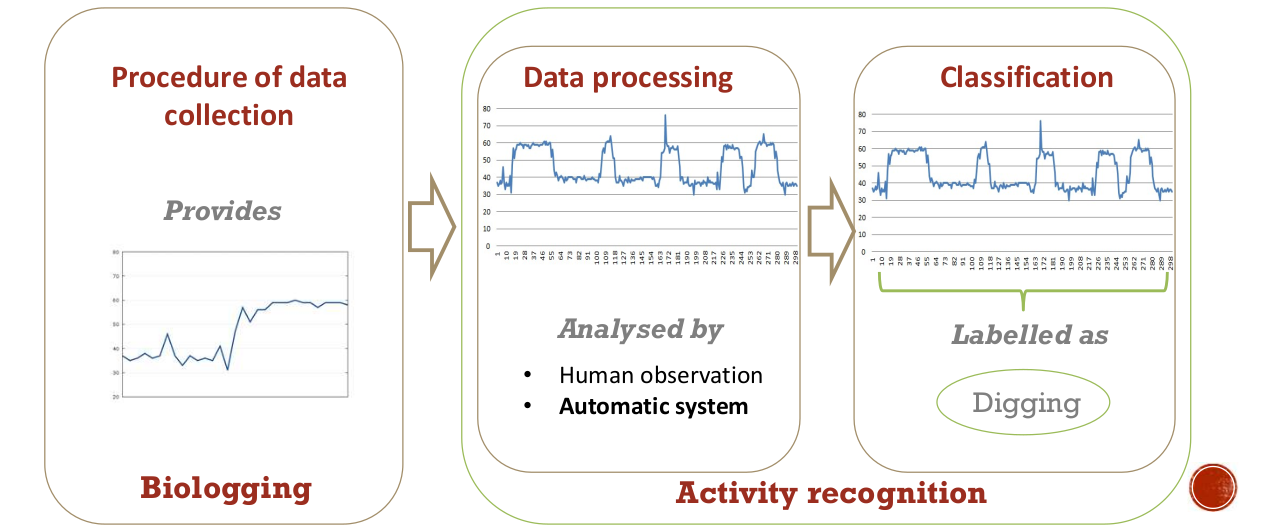
\includegraphics{images/biologging_processing.png}
   \caption{Biologging data lifecycle.}
   \label{fig:biologging_processing}
   Biologging provides raw data which is later processed and classificated.
\end{figure}

% \begin{paracol}{2}
   
%    \labelitemize{\color{darkgreen}\ul{\textit{Strengths}}}{
%       \color{darkgreen}
%    }
%    \switchcolumn
%    \labelitemize{\color{darkred}\ul{\textit{Strengths}}}{
%       \color{darkred}
%    }

% \end{paracol}

\proscons{Strengths}{Weaknesses}{
   \begin{itemize}
      \item Data are punctual observations collected through sensors; 
      \item Observation in both domestic and wild environments
      \item Availability of a huge amount of data (time-series data) 
      \item Although this requires suitable data analysis algorithms.
   \end{itemize}
}{
   \begin{itemize}
      \item Need to attach the device to the subject;  
      \item Need to physically retrieve the device 
      \item When the memory fills up or battery drains out  
      \item Device lifetime in battery- intensive monitoring 
      \item Often off-line analysis 
   \end{itemize}
}

\section{Device perspective}
The common sense may lead to an approach involving a  collector device having a low power logger which produces ---huge amounts of--- time series data, which then should either send the data to a remote station, or to be physically retrieved to download the time series data.\\
In case of \ul{biologging both options are typically not feasible}, because sending data considerably reduces the battery life, and retrieving the device from the back of an elephant is a risky and surely not easy task. \smiley

A more \textit{novel approach} consists in \textbf{embedding} the automatic classifier on-board, and store and trasmit only the results of classification obtaining both memory and communication efficiency, at the cost of computing power.

\section{Tortoises case study}

\textit{``Localizing tortoise nests by neural network''} is a study published by Chessa et. al in 2016.
The \textbf{motivation} for the study was that Protection programs of tortoises aim at retrieving the eggs and bringing them at a protection center, where hatchlings are protected during their most vulnerable period, while the \textbf{problem} to overcome was that the identification of tortoise nests in wild is usually very challenging, as tortoises are extremely good in hiding them.

The study aimed to localize the nests of tortoises by using a neural network classifier, which was trained on the data collected by a device attached to the tortoises. The device was equipped with a GPS and an accelerometer, and was able to collect data on the tortoise's movements. The classifier was trained to recognize the patterns of movement associated with the construction of a nest, and was able to accurately predict the location of the nest based on the data collected by the device.

\textit{Tortoise@} ---the designed classifier's name--- is structured as depicted in the Fig \ref{fig:tortoise@_architecture} below.
\begin{figure}[htbp]
   \centering
   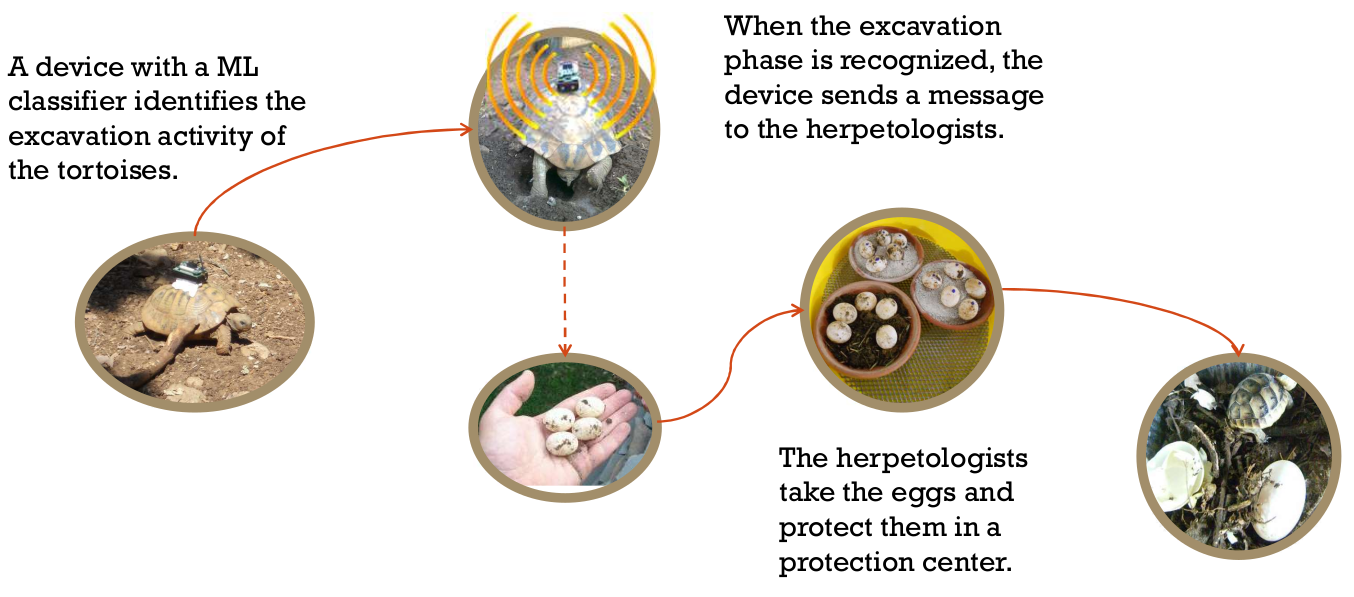
\includegraphics{images/tortoise@_architecture.png}
   \caption{Tortoise@ architecture}
   \label{fig:tortoise@_architecture}
\end{figure}

\subsection{What about tortoise nests?}
\framed{
   \begin{itemize}
      \item Tortoises lay eggs in spring (over 4 months)
      \item A single tortoise may lay eggs more than once (generally up to three/four times)
      \item Nesting happens at daytime, in warm and well-lit places
      \item Nesting lasts for more than one hour
      \item The tortoises digs their nests with their hind paws
   \end{itemize}
   \begin{enumerate}
      \item[] \textbf{Hence}:
      \item The device lifetime must be at least 4 months
      \item Digging activity indicates a probable nesting: it can be detected with accelerometers, because the tortoise moves its legs in a peculiar way, and initiating a nest takes about 90 seconds. However, not all the digging activities are related to nesting.
      \item Use of environmental sensors (light and temperature) to limit the use of accelerometers, because without specific environmental conditions the tortoise will not nest, so it is not necessary to spend energy in that period of time.
   \end{enumerate}
   }

   \subsection{Data collection and processing}
   The dataset was collected at the ``Centro di protezione tartarughe meditarrenee'' at Massa Marittima in Italy, and was made up of raw time-series from an accelerometer.
   Such raw data was processed to build a Sequences datasets and a Patterns dataset.
   \begin{figure}[htbp]
      \centering
      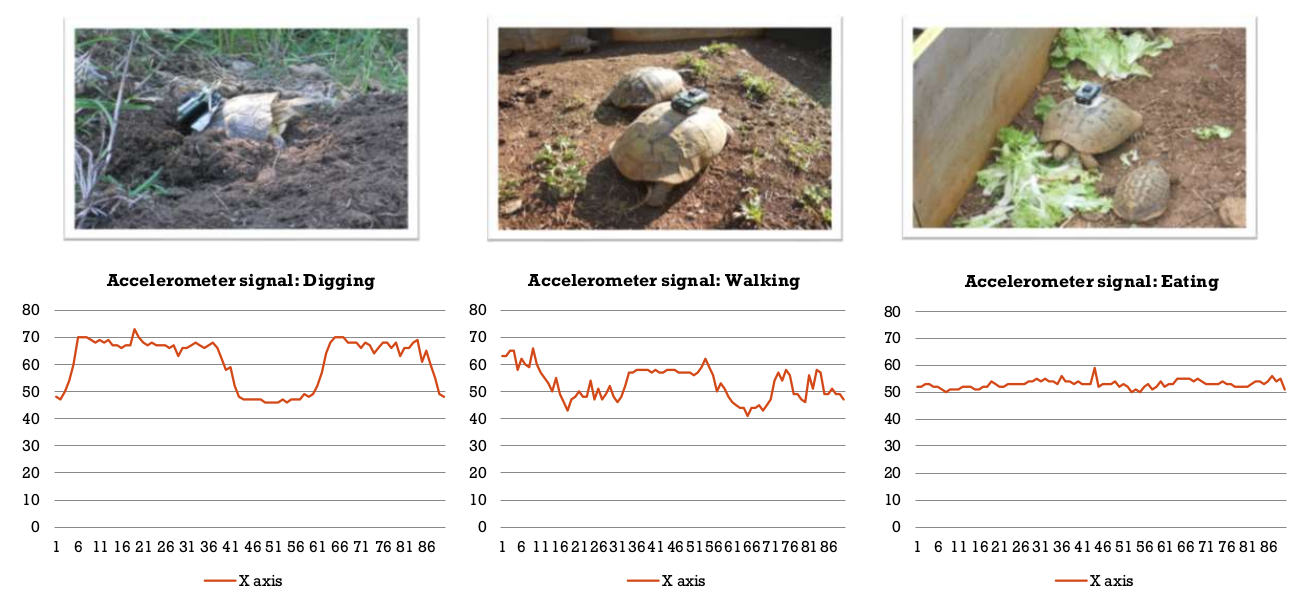
\includegraphics{images/tortoise@_accelerometer.png}
      \caption{Tortoise activities and accelerometer data}
      \label{fig:tortoise@_accelerometer}
   \end{figure}

\begin{paracol}{2}
   

   The use of SVM and of several models of neural networks (ESN, IDNN, CNN) are considered. Two approaches may be adopted:
   \begin{enumerate}
      \item \textbf{Asynchronous tasks}: classification of single windows. (\note{IDNN, CNN, SVM, ESN})
      \note{The output of the neural network depends on an entire window}
      \item \textbf{Synchronous tasks}: classification in step by step across a stream of data. (\note{ESN})
      \note{The output of the neural network does not need an entire window of samples.  It is based on the samples of the last 90 seconds (sufficient to find a pattern)}
   \end{enumerate}
   
   \switchcolumn

   \begin{figure}[htbp]
      \centering
      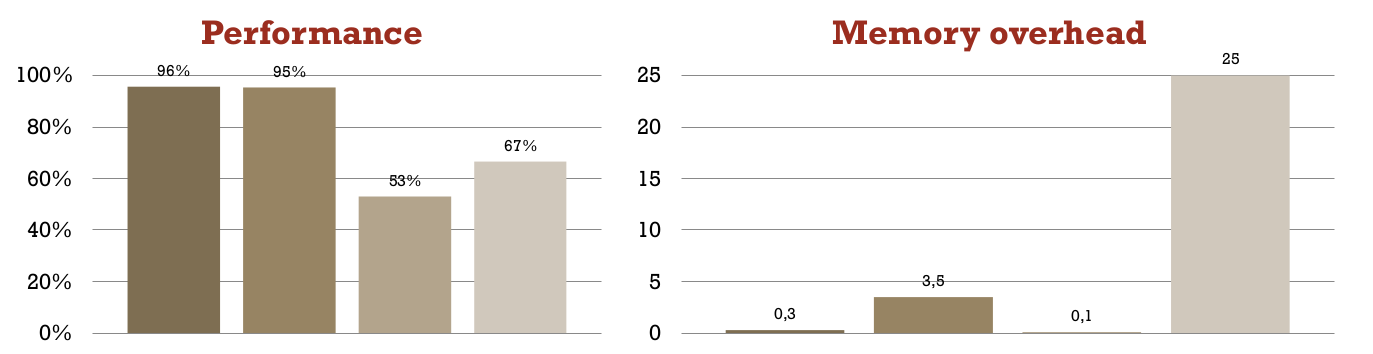
\includegraphics{images/tortoise@_modelcomparison.png}
      \caption{Models comparison for \textit{Asynchronous tasks}}
      \label{fig:tortoise@_modelcomparison}
      The hardware used was an Arduino equivalent, with a 16 MHz clock and \textbf{4 KB} of RAM, which made some of the displayed model completely unfeasible.
   \end{figure}
\end{paracol}

Energy consumption must be clearly taken into account when establishing the sampling frequency, and some assumptions helped achieving efficiency, such as avoiding sampling at night, or when environmental conditions are not suitable for nesting.\\
Also the data structures required by the models must be taken into account, as they may require a lot of memory, which is a scarce resource in the device.
\note{Only two main data structures were used, one to store the activity recognition machine and another to store acceleration samples.}

\framedt{Cloud vs Local processing}{
Cloud processing implies:
\begin{itemize}
   \item Store (and transmit) GPS position every half an hour (two long, 32 bits each)
   \item Store (and transmit) the acceleration data sampled at 1Hz (10 bits each sample)
   \item For 4 months continuously: 46 KBytes (GPS) + 13 Mbytes (accelerometer)
\end{itemize}

Local processing implies instead:
\begin{itemize}
   \item \textbf{Transmit} GPS position: 32 bits latitude, 32 bits longitude only when detected excavation
   \note{Occurs only a few times in 4 months (not all excavations conclude with nesting)}
   \item \textbf{Storage}:
   \begin{itemize}
      \item Accelerometer data: at most 3 KBytes (a time window), even less with ESN
      \item GPS: only when detects excavation
   \end{itemize}
\end{itemize}
   }